\documentclass[a4paper, twoside]{report}

%% Language and font encodings
\usepackage[english]{babel}
\usepackage[utf8x]{inputenc}
\usepackage[T1]{fontenc}

%% Sets page size and margins
\usepackage[a4paper,top=3cm,bottom=2cm,left=3cm,right=3cm,marginparwidth=1.75cm]{geometry}

%% Useful packages
\usepackage{amsmath}
\usepackage{amssymb}
\usepackage{amsthm}
\usepackage{graphicx}
\usepackage[colorinlistoftodos]{todonotes}
\usepackage[colorlinks=true, allcolors=blue]{hyperref}

% Define theorem-like environments
\newtheorem{theorem}{Theorem}[section] % Theorems numbered within sections
\newtheorem{corollary}[theorem]{Corollary} % Corollaries share numbering with theorems
\newtheorem{lemma}[theorem]{Lemma} % Lemmas share numbering with theorems

% Define definition-like environments
\theoremstyle{definition}
\newtheorem{definition}{Definition}[section] % Definitions numbered within sections
\newtheorem{algorithm}[definition]{Algorithm}

% Define observation environment
\newtheorem{observation}{Observation}[section] % Observations numbered within sections

% Define remark-like environment
\theoremstyle{remark}
\newtheorem{remark}{Remark}[section] % Remarks numbered within sections

\newtheorem{exercise}{Exercise}[section]
\newtheorem*{solution}{Solution}

\newcommand{\legendre}[2][p]{\ensuremath{\left( \dfrac{#2}{#1} \right) }}

\title{Note}
\author{John Smith}
% Update supervisor and other title stuff in title/title.tex

\begin{document}
\begin{titlepage}

  \newcommand{\HRule}{\rule{\linewidth}{0.5mm}} % Defines a new command for the horizontal lines, change thickness here
  
  %----------------------------------------------------------------------------------------
  %	LOGO SECTION
  %----------------------------------------------------------------------------------------
  
  %\includegraphics[width=8cm]{title/logo.eps}\\[1cm] % Include a department/university logo - this will require the graphicx package
   
  %----------------------------------------------------------------------------------------
  
  \center % Center everything on the page
  
  %----------------------------------------------------------------------------------------
  %	HEADING SECTIONS
  %----------------------------------------------------------------------------------------
  
  \textsc{\LARGE Individual}\\[1.5cm] % Name of your university/college
  \textsc{\Large Number Theory, Topology, Real and Complex Analysis}\\[0.5cm] % Major heading such as course name
  \textsc{\large Individual Project during 2023 Summer}\\[0.5cm] % Minor heading such as course title
  
  %----------------------------------------------------------------------------------------
  %	TITLE SECTION
  %----------------------------------------------------------------------------------------
  \makeatletter
  \HRule \\[0.4cm]
  { \huge \bfseries \@title}\\[0.4cm] % Title of your document
  \HRule \\[1.5cm]
   
  %----------------------------------------------------------------------------------------
  %	AUTHOR SECTION
  %----------------------------------------------------------------------------------------
  
  %\begin{minipage}{0.4\textwidth}
  %\begin{flushleft} \large
  %\emph{Author:}\\
  %\@author % Your name
  %\end{flushleft}
  %\end{minipage}
  %~
  %\begin{minipage}{0.4\textwidth}
  %\begin{flushright} \large
  %\emph{Supervisor:} \\
  %Prof. Lily Smith \\[1.2em] % Supervisor's Name
  %\emph{Second Marker:} \\
  %Dr. Adam Smith % second marker's name
  %\end{flushright}
  %\end{minipage}\\[2cm]
  %\makeatother
  
  % If you don't want a supervisor, uncomment the two lines below and remove the section above
  \Large \emph{Author:}\\
  Hyunjun \textsc{Choi}\\[3cm] % Your name
  
  %----------------------------------------------------------------------------------------
  %	DATE SECTION
  %----------------------------------------------------------------------------------------
  
  {\large \today}\\[2cm] % Date, change the \today to a set date if you want to be precise
  
  \vfill % Fill the rest of the page with whitespace
  
  \end{titlepage}

\tableofcontents
\listoffigures
\listoftables

\chapter{Introduction}
A solid foundation in mathematics, including number theory, topology, real and  complex analysis, is of paramount importance for individuals pursuing studies in natural sciences and engineering. This article is written at the request of my friend, an enthusiastic physicist and a Pleiades cluster lover, who currently is serving for obligatory military service, but wants to keep track of his study. However, I hope this article serves as a helpful resource for students, future or current researchers, and enthusiasts in various fields, including natural sciences and engineering. \\
Though I said that solid foundation in mathematics is important, this article is not mathematically strict. Of course I provide proofs for important theorems or features, but it omits a lot of proofs. The aim of this article is not to be a lecture note for students, but to provide intuition or serve as a cheat sheet.
\cite{temporary02}
\chapter{Number Theory}

\section{Pythagorean Triples}

A \textbf{Primitive Pythagorean Triple (PPT)} is a tuple $(a, b, c)$ where $a$, $b$, $c$ have no common factors and satisfy $a^{2}+b^{2}=c^{2}$. It has few features:

\begin{observation}
One of $a$ \& $b$ is odd and the other even, so $c$ is always odd.
\end{observation}

\begin{observation}
If $(a, b, c)$ is PPT, then we can factor $a^{2}=c^{2}-b^{2}$. It looks like $c - b$ and $c + b$ are themselves always squares and have no common factors.
\end{observation}

\begin{proof}
I first prove that $gcd(c - b, c + b) = 1$. \\
Let $d = gcd(c - b, c + b)$. \\ 
Then $c - b = dk$, $c + b = dl$, $k,l\in \mathbb{N}$. \\
Since $2b = d(l - k)$ and $2c = d(l + k)$, $d\mid gcd(2b, 2c)$. \\
Now suppose $gcd(b, c)= g > 1$. \\
Set $b = g\tilde{b}$, $c = g\tilde{c}$. \\
Then $a^{2} = g^{2}(\tilde{c}^{2} - \tilde{b}^{2})$, which leads to $g\mid a$. \\
However, this is a contradiction by \textbf{Observation 2.1.1}. \\
Thus, $gcd(b, c) = 1$ and $gcd(2b, 2c) = 2$. \\
We now know that $d = 1$ or $d = 2$ as $d \mid gcd(2b, 2c)$. \\
If $d = 2$, then $a^{2}=(c-b)(c+b)=4kl$ so $2\mid a$, which is again a contradiction. \\
Thus $d = 1$.\\
\\
Now I prove $c - b$ and $c + b$ are squares. \\
Let $a = p_{1}^{n_{1}}\dots p_{r}^{n_{r}}$ where $p_{i}$ prime, $n\in \mathbb{N}$. \\
Then $a^{2} = p_{1}^{2n_{1}}\dots p_{r}^{2n_{r}} = (c - b)(c + b)$. \\ 
As $gcd(c - b, c + b) = 1$ by \textbf{Observation 2.1.1}, they are squares.
\end{proof}

\noindent
A \textbf{Primitive Pythagorean Pair (PPP)} is a pair $(s, t)$ s.t. $a = st$, $b = \dfrac{s^{2} - t^{2}}{2}$, $c = \dfrac{s^{2} + t^{2}}{2}$. \\
We can induce it by substituting $c + b = s^{2}$, $c - b = t^{2}$. \\
\\
It is worth noting the relationship between the PPT and unit circle. We start by dividing the both sides of $a^{2} + b^{2} = c^{2}$ by $c^{2}$. Then we can induce the typical unit circle form by substituting as $x = \dfrac{a}{c}$ and $y = \dfrac{b}{c}$. Our goal is to find $(x, y)$ where $x, y\in \mathbb{Q}$.

\begin{figure}[h]
\caption{A Unit Circle and a line passing through (-1, 0)}
\centering
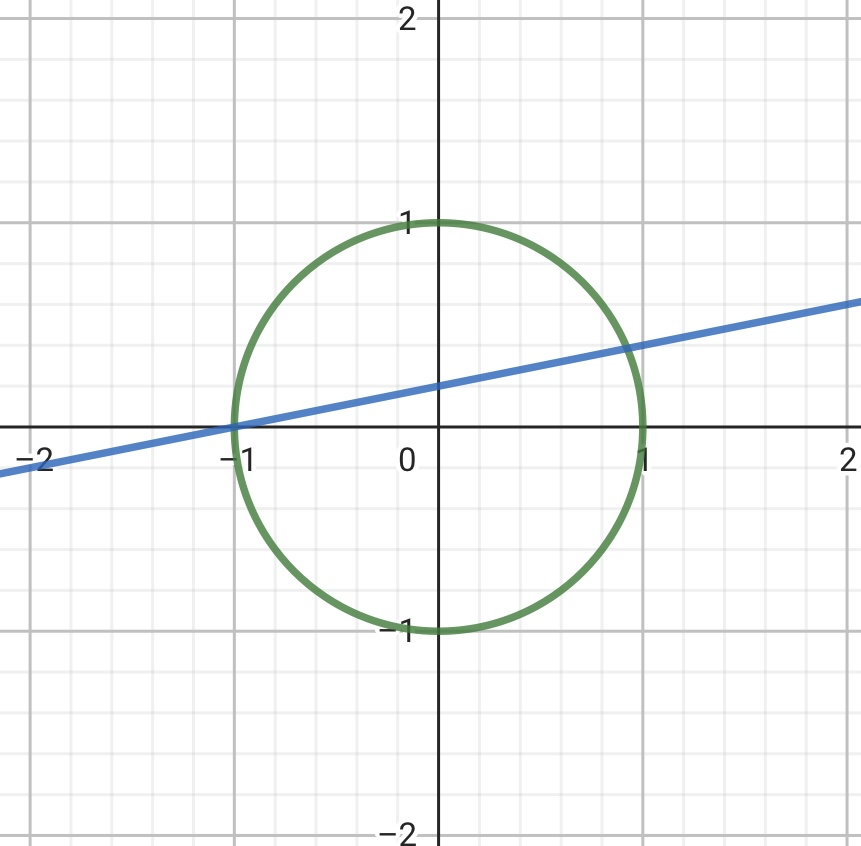
\includegraphics[width=0.5\textwidth]{number_theory/fig2-1.jpg}
\end{figure}

We find by exploiting geometry. As we know the trivial solution $(-1, 0)$, we draw a line that passes through $(-1, 0)$ and get the coordinate of the intersection other than $(-1, 0)$. We set the slope of the line $m\in \mathbb{Q}$ so that all the intersections are of $\mathbb{Q}\times \mathbb{Q}$. 
\begin{align*}
x^{2} + m^{2}(x + 1)^{2} &= 1
(1 + m^{2})x^{2} + 2m^{2}x + (m^{2} - 1) &= 0
(x, y) &= (\frac{1 - m^{2}}{1 + m^{2}}, \frac{2m}{1 + m^{2}})
\end{align*}

Now let $m = \dfrac{v}{u}$ as $m\in \mathbb{Q}$. Then we can finally induce another way to describe Pythagorean triples: $(a, b, c) = (u^{2} - v^{2}, 2uv, u^{2} + v^{2})$. This is equivalent form when $u = \dfrac{s + t}{2}$, $v = \dfrac{s - t}{2}$. Note that not all $u$, $v$ give us PPT.
\section{Euclidean Algorithm}

\begin{theorem}[Euclidean Algorithm]
Let $r_{-1} = a$, $r_{0} = b$, $r_{i - 1} = q_{i + 1}r_{i} + r_{i + 1}$, $i = 0, 1,\dots$ until $r_{n + 1} - 0$. Then $r_{n} = gcd(a, b)$.
\end{theorem}

\begin{proof}
We inspect the last iteration: $r_{n - 1} = q_{n + 1}r_{n} + 0$. \\
We observe that $r_{n}\mid r_{n - 1}$. \\
Now, inspect the penultimate iteration: $r_{n - 1} = q_{n}r_{n - 1} + r_{n}$. \\
We observe that $r_{n}\mid r_{n - 2}$. \\
Iterating through, we get $r_{n}\mid r_{0}$ and $r_{n}\mid r_{-1}$. \\
Hence, $r_{n}$ is a common divisor of $a$ and $b$. \\
To prove that $r_{n} = gcd(a, b)$, suppose that $gcd(a, b) = d$. \\
By the definition of gcd, $d\mid a$ and $d\mid b$. \\
We inspect the first iteration: $a = q_{1}b + r_{1}$. \\
We observe that $d\mid r_{1}$
Iterating through, we get $d\mid r_{n}$. Hence, we conclude that $d = r_{n}$.
\end{proof}

Euclidean Algorithm has some features:

\begin{observation}
Let $b = r_{0}, r_{1}, \dots$ be the successive remainders in Euclidean algorithm applied to $a$ and $b$. For every two steps, the remainder is reduced by at least one half: $r_{i + 2} < \dfrac{1}{2}r_{i}$, $i = 0, 1, \dots$.
\end{observation}

\begin{observation}
The algorithm terminates in at most $2\log_{2}b$ steps. In particular, the number of steps is at most seven times the number of digits of $b$.
\end{observation}

\noindent
I omit the proofs. \\
Finally, it is worth noting that $gcd(a, b)\times lcm(a, b) = ab$.
\section{Properties of ax + by = c}

\begin{theorem}[Linear Equation Theorem]
  The equation $ax + by = c$ has integer solution pairs if and only if $gcd(a, b)\mid c$. The solution is expressible by $(x_{1} + \dfrac{kb}{g}, y_{1} - \dfrac{ka}{g})$ where $k\in \mathbb{Z}$, $(x_{1}, y_{1})$ a trivial solution.
\end{theorem}

\noindent
To prove it, apply Euclidean algorithm. I omit the specifics.
\section{Congruences}

\begin{definition}
  $a$ is congruent to $b$ modulo m if $m\mid a - b$ and denote $a\equiv b\; (\bmod{m})$
\end{definition}

\noindent
It is noteworthy to mention some properties:

\begin{observation}
  If $a_{1}\equiv b_{1}\; (\bmod{m})$ and $a_{2}\equiv b_{2}\; (\bmod{m})$, then $a_{1} \pm a_{2}\equiv b_{1}\pm b_{2}\; (\bmod{m})$ and $a_{1}a_{2}\equiv b_{1}b_{2}\; (\bmod{m})$.
\end{observation}

\begin{observation}
  If $ac\equiv bc\; (\bmod{m})$, it need not be true that $a\equiv b\; (\bmod{m})$. If, however, $gcd(c, m) = 1$, it is always true. 
\end{observation}

\noindent
Now I should introduce a technique which we will (hopefully) love. \\
A \textbf{Climb Every Mountain Technique} is, when solving a congruence modulo $m$, we try each value $0, 1, \dots m - 1$. I would say this technique, in Korean, as No-ga-da. This technique is often useful and is only the technique you can use. For example, to solve $x$ such that $x^{2}\equiv 3\; (\bmod{10})$, we substitute $0\dots 9$ to $x$ and find out there is no solution.

\begin{theorem}[Linear Congruence Theorem]
  Let $a, c, m\in \mathbb{Z}$ with $m\geq 1$ and let $g = gcd(a, m)$. \\
  (1) If $g\nmid c$, then $\nexists{x}$ s.t. $ax\equiv c\; (\bmod{m})$. \\
  (2) If $g\mid c$, then $ax\equiv c\; (\bmod{m})$ has exactly $g$ in congruent solutions.
\end{theorem}

\begin{proof}
Proof for (1). \\
Suppose $\exists{x_{0}}$ such that $ax_{0}\equiv c\; (\bmod{m})$ when $g\nmid c$. \\
Then $\exists{y}$ such that $ax_{0} + my = c$. \\
Now observe that $g\mid a$ thus $g\mid ax_{0}$ and $g\mid m$ thus $g\mid my$. \\
Then $g\mid c$ should satisfy, and this is a contradiction. \\
I omit the proof for (2).
\end{proof}

Arguably, the most important case of \textbf{Linear Congruence Theorem} is when $gcd(a, m) = 1$: $ax\equiv c\; (\bmod{m})$. In this case, it has only one solution and denote it as $x\equiv a^{-1}c\; (\bmod{m})$. \\
\\
I lastly mention \textbf{Polynomial Roots Mod} $p$ \textbf{Theorem} and finish this section.

\begin{theorem}
(Polynomial Roots Mod $p$ Theorem) \\
Let $p$ be a prime number and let $f(x) = a_{0}x^{d} + a_{1}x^{d - 1} + \cdots + a_{d}$ be a polynomial of degree $d\geq 1$ with integer coefficients and with $p\nmid a_{0}$. Then $f(x)\equiv 0\pmod{p}$ has at most $d$ incongruent solutions.
\end{theorem}

\noindent
I omit the proof.
\section{Fermat's Little Theorem}

\begin{lemma}
Let $a\not\equiv 0\; (\bmod{p})$. $\{a, 2a,\cdots (p - 1)a \; (\bmod{p})\} = \{1, 2,\cdots (p - 1) \; (\bmod{p})\}$
\end{lemma}

\begin{proof}
  Note that for $1\geq k\geq p - 1$, $ka\not\equiv 0\; (\bmod{p})$. \\
  Thus, it is sufficient to show that for $1\geq i < j\geq p - 1$, $ia\not\equiv ja\; (\bmod{p})$. \\ 
  By the assumptions, $j - i\not\equiv 0\; (\bmod{p})$ and $a\not\equiv 0\; (\bmod{p})$, so $(j - i)a\not\equiv 0\; (\bmod{p})$. \\
  Thus $i\neq j$ and $ia\not\equiv ja\; (\bmod{p})$ is a bijection.
\end{proof}

\begin{theorem}[Fermat's Little Theorem]
  Let $p$ be a prime number and $a$ be any number with $a\not\equiv 0\; (\bmod{p})$. Then $a^{p - 1}\equiv 1\; (\bmod{p})$.
\end{theorem}

\begin{proof}
  $a\times 2a\dots (p - 1)a = (p - 1)!a^{p - 1}$. \\
  By Lemma, $(p - 1)!a^{p - 1}\equiv (p - 1)!\; (\bmod{p})$. \\
  Hence, $a^{p - 1}\equiv 1\; (\bmod{p})$.
\end{proof}

Suppose that we want to calculate $11^{104}\; (\bmod{17})$. We know, by \textbf{Fermat's Last Theorem}, that $11^{16}\equiv 1\; (\bmod{17})$. Thus $11^{96}\equiv 1\; (\bmod{17})$ and $11^{104}\equiv 11^{8}\; (\bmod{17})$. We can then exploit the fact that $11^{8} = (11^{2})^{4}$. Since $11^{2}\equiv 2\; (\bmod{17})$, we know that $11^{8}\equiv 16\equiv -1\; (\bmod{17})$.

\begin{theorem}[Wilson's Theorem]
  For a prime number $p$, $(p - 1)!\equiv -1\; (\bmod{p})$.
\end{theorem}

\begin{proof}
We first look for trivial cases: when $p = 2,3$. The theorem holds. \\
For $p > 3$, it is sufficient to show that $2\times \dots (p - 2)\equiv 1\; (\bmod{p})$. \\
To show, we look the features of $ax\equiv 1\; (\bmod{p})$. \\
As $gcd(a, p) = 1$, there always exists a unique $x$; say this $a'$.
If $a = a'$, then $a'\equiv 1\; (\bmod{p})$ or $a'\equiv -1\; (\bmod{p})$ as 
\begin{align*}
aa' &\equiv 1\; (\bmod{p}) \\
a^{2} &\equiv 1\; (\bmod{p}) \\
(a - 1)(a + 1) &\equiv 0\; (\bmod{p})
\end{align*}
If $a\neq a'$, then we can always find a pair $(a, a')$ that satisfies $aa'\equiv 1\; (\bmod{p})$ by the guaranteed existence and uniqueness of $a'$. \\
\\
By the case of $a\neq a'$ above, we notice $(p - 2)!\equiv 1\; (\bmod{p})$.
\end{proof}
\section{Euler's Formula}

The shortcoming of \textbf{Fermat's Little Theorem} is that it only works for prime number. However, we are also interested in $k$s when given some composite number $m$ and a number $a$ that satisfies $a^{k}\equiv 1\; (\bmod{m})$. From the previous knowledge, such is only possible when $gcd(a, m) = 1$. Thus, it is natural to look at the set of numbers that are relatively prime to $m$.

\begin{definition}[Euler's Phi Function]
  $\phi(m) = |\{a: 1\geq a\geq m,\; gcd(a, m) = 1\}|$.
\end{definition}

One important feature of Euler's phi function is that, for a given prime number $p$, $\phi(p) = p - 1$ as every integer $1\geq a < p$ is relatively prime to $p$. Also, $\phi(p^{k}) = p^{k} - p^{k - 1}$.

\begin{theorem}[Euler's Formula]
  If $gcd(a, m) = 1$, then $a^{\phi(m)}\equiv 1\; (\bmod{m})$.
\end{theorem}

\begin{proof}
The logic behind the proof is similar to that of \textbf{Fermat's Little Theorem}.
\end{proof}

\begin{theorem}
If $gcd(m, n) = 1$, then $\phi(mn) = \phi(m)\phi(n)$.
\end{theorem}

\begin{proof}
Define $A = \{a: 1\leq a\leq mn, \; gcd(a, mn) = 1\}$ \\
$B = \{(b, c): 1\leq b\leq m, \; 1\leq c\leq n,\; gcd(b, m) = gcd(c, n) = 1\}$. \\
Note that $|A| = \phi(mn)$, $|B| = \phi(m)\phi(n)$. \\
Now, let $f: A\to B$. It is sufficient to show that $f$ is bijective. In fact, this is implied by \textbf{Chinese Remainder Theorem}.
\end{proof}

\begin{theorem}[Chinese Remainder Theorem]
Let $m, n$ be integers such that $gcd(m, n) = 1$. Let $b$ ($0\leq b\leq m$) and $c$ ($0\leq c\leq n - 1$) be any integers. Then $x\equiv b\; (\bmod{m})$ and $x\equiv c\; (\bmod{n})$ have exactly one solution where $0\leq x < mn$.
\end{theorem}

I omit the proof for \textbf{Chinese Remainder Theorem}. Instead, I give an example written on Sunzi Suanjing: \\
\textit{We have a number of things, but we do not know exactly how many. If we count them by threes, we have the two left over. If we count them by fives, we have three left over. If we count them by sevens, we have two left over. How many things are there?} \\
We are given that $x\equiv 2\; (\bmod{3})$, $x\equiv 3\; (\bmod{5})$, $x\equiv 2\; (\bmod{7})$. \\
As $3, 5, 7$ are pairwise relatively prime, the given system of congruences have exactly one solution for modulus 105 by \textbf{Chinese Remainder Theorem}. \\
We set $x\equiv 35a_{1} + 21a_{2} + 15a_{3}\; (\bmod{105})$. Now our goal is to find $a_{1},a_{2},a_{3}$ such that $35a_{1}\equiv 2\; (\bmod{3})$, $21a_{2}\equiv 3\; (\bmod{5})$, $15a_{3}\equiv 2\; (\bmod{7})$. \\
I first find $a_{1}$:
\begin{align*}
  35a_{1} &\equiv 2\; (\bmod{3}) \\
  35\cdot 2\cdot a_{1}' &\equiv 2\; (\bmod{3})
\end{align*}
Now my goal is to find $a_{1}'$ such that $35a_{1}'\equiv 1\; (\bmod{3})$. \\
As $a_{1}'\equiv 35^{-1}\; (\bmod{3})$, $a_{1}' =  1$ thus $a_{1} = 2$. \\
By the similar logic, $a_{2} = 1$, $a_{3} = 1$. \\
Thus, $x\equiv 23\; (\bmod{105})$.
\section{Infinite Primes}

I start by introducing \textbf{Prime Divisibility Theorem} and the \textbf{Fundamental Theorem of Arithmetic}.

\begin{theorem}[Prime Divisibility Theorem]
Suppose that for some prime $p$, if $p\mid a_{1}a_{2}\cdots a_{r}$ where $a_{1}a_{2}\cdots a_{r}\in \mathbb{Z}_{\geq 2}$, $r\in \mathbb{Z}_{\geq 2}$, then $1\leq \exists i\leq r$, $p\mid a_{i}$.
\end{theorem}

\noindent
I omit the proof.

\begin{theorem}[The Fundamental Theorem of Arithmetic]
All natural numbers larger than 1 can be factored into the product of primes in exactly one way.
\end{theorem}

\begin{proof}
I first prove the existence of the factorisation. I prove by induction. \\
We check the base case: the theorem holds in case of $2$. \\
We check the inductive case: assume that for $2\leq \forall n\leq k$, $\forall k\in \mathbb{Z}_{\geq 2}$ the theorem holds. \\
If $n = k + 1$ is prime, the theorem holds. \\
If $n = k + 1$ is composite, then we can factorise as $n = n_{1}n_{2}$ where $2\leq n_{1}, n_{2}\leq k$. \\
By assumption, $n_{1}, n_{2}$ can be facotored into the product of primes, so $n$ can. \\
\\
Now I prove the uniqueness of factorisation. \\
Suppose there are more than one way of factorisation: $n = p_{1}p_{2}\cdots p_{r} = q_{1}q_{2}\cdots q_{s}$. \\
Without loss of generality, say that $p_{1}p_{2}\cdots p_{r}$ and $q_{1}q_{2}\cdots q_{s}$ does not have common factor. \\
If they have some, simply erase them and acquire the same form. \\
Now look $p_{1}$. Since $p_{1}\mid p_{1}p_{2}\cdots p_{r} = n$, $p_{1}\mid q_{1}q_{2}\cdots q_{s}$. \\
Then, by \textbf{Prime Divisibility Theorem}, $1\leq \exists i\leq s$, $p_{1}\mid q_{i}$. Contradiction.
\end{proof}

\begin{theorem}
There are infinitely many primes.
\end{theorem}

\begin{proof}
  Suppose there are finite number of primes. \\
  Name each as $p_{1}, p_{2},\dots p_{n}$ where $n$ is the number of primes. \\
  Now we inspect the number $x = p_{1}p_{2}\cdots p_{n} + 1$. \\
  We observe that $x$ is a composite number as it is not one of the primes we pre-defined. \\
  Since $x$ is a composite number, according to \textbf{Fundamental Theorem of Arithmetic}, there must exist some prime number $p$ such that $p\mid x$. \\
  However, we observe there is no such prime number in our predefined prime numbers that can factorise $x$. This is a contradiction as, according to \textbf{Fundamental Theorem of Arithmetic}, all number should be factorised into the product of prime numbers. $x$ is a composite number, so there must exist some prime that can factorise $x$.
\end{proof}

\noindent
I provide an example regarding \textbf{Theorem 2.7.3} and generalise later to \textbf{Dirichlet's Theorem on Primes in Arithmetic Progressions}. 

\begin{exercise}
Show that there are infinitely many primes that are congruent to $5 \pmod{6}$.
\end{exercise}

\begin{solution}
Suppose that $ps = \{5, p_{1}, p_{2}\dots p_{n}\}$ be the finite primes which are congruent to 5 mod 6. \\
We inspect the number $x = 6p_{1}p_{2}\cdots p_{n} + 5$. \\ 
First observe that $x\equiv 5 \pmod{6}$. Since $x$ is not in pre-defined set $ps$, $x$ is composite. \\
Then, by \textbf{Fundamental Theorem of Arithmetic}, we can factorise $x$ into product of primes: $x = q_{1}q_{2}\cdots q_{r}$ where all $q$s are primes. \\
Now, observe that $3\nmid x$. Thus, $x = 6k + 1$ or $x = 6k + 5$. \\
Now we look at the features of $q$s. \\
If $\forall i$ $q_{i}\equiv 1 \pmod{6}$, then $x = q_{1}\cdots q_{r}\equiv 1 \pmod{6}$. We can thus know that at least one $q$ is $\equiv 5 \pmod{6}$. Say such $q$ as $q'$. \\
Then $q'\in ps$ as $ps$ contain all the primes that is $\equiv 5 \pmod{6}$. \\
If $q' = 5$, then $5\mid x$. Contradiction. \\
If $q' = p_{t}$, $1\leq t\leq n$, then $q'\mid 6p_{1}p_{2}\cdots p_{r}$ and $q'\mid x$. \\
So $q'\mid 5$, which is a contradiction.
\end{solution}

\begin{theorem}[Dirichlet's Theorem on Primes in Arithmetic Progressions]
Let $a, m\in \mathbb{Z}$, $gcd(a, b) = 1$. Then there are infinitely many primes that are congruent to $a \pmod{m}$.
\end{theorem}

\noindent
I omit the proof. \\
\\
Finally, I mention \textbf{Prime Number Theorem} and move on to next section.

\begin{theorem}[The Prime Number Theorem]
When $x\in \mathbb{Z}$ is large, the number of primes less than $x$ is approximately equal to $\dfrac{x}{ln{x}}$
\end{theorem}
\section{$k$th Powers Modulo $m$ and $k$th Roots Modulo $m$}

Our goal is to compute $k$th powers modulo $m$ when $k$ and $m$ are very large. 

\begin{algorithm}
(Successive Squaring to Compute $a^{k} \pmod{m}$)
\begin{enumerate}
\item Write $k$ as a sum of powers of $2$, $k = u_{0} + u_{1}\cdot 2 + u_{2}\cdot 2^{2} + \cdots$, where each $u_{i}$ is either $0$ or $1$. (binary expansion of $k$.)
\item Make a table of powers of $a$ modulo $m$ using successive squaring. \\
$a^{1}\equiv A_{0}\pmod{m}$ \\
$a^{2}\equiv A_{0}^{2}\equiv A_{1}\pmod{m}$ \\
\vdots \\
$a^{2^{r}}\equiv A_{r - 1}^{2}\equiv A_{r}\pmod{m}$
\item The product $A_{0}^{u_{0}}\cdot A_{1}^{u_{1}}\cdots A_{r}^{u_{r}}\pmod{m}$ will be congruent to $a^{k}\pmod{m}$. 
\end{enumerate}
\end{algorithm}

\noindent
As an example, I compute $2^{9990}\pmod{9991}$. \\
First, I convert 9990 to binary: $9990 = 2^{13} + 2^{10} + 2^{9} + 2^{8} + 2^{2} + 2^{1}$. \\
Then, I look at the able of powers of $2$ modulo $m$:
\begin{table}[h!]
\centering
\begin{tabular}{||c c c c c c c||} 
  \hline \hline
  $2^{1}$ & $2^{2}$ & $2^{4}$ & $2^{8}$ & $2^{16}$ & $2^{32}$ & $2^{64}$ \\
  \hline
  2 & 4 & 16 & 256 & 5590 & 6243 & 158 \\ 
  \hline \hline
  $2^{128}$ & $2^{256}$ & $2^{512}$ & $2^{1024}$ & $2^{2048}$ & $2^{4096}$ & $2^{8192}$ \\
  \hline
  4982 & 2680 & 8862 & 5784 & 4788 & 5590 & 6243 \\
  \hline \hline
\end{tabular}
\caption{Table of Powers of $2$ modulo $m$}
%% \label{table:1}
\end{table}
\noindent
Finally, 
\begin{align*}
2^{9990} &\equiv 6243\cdot 5784\cdot 8862\cdot 2680\cdot 16\cdot 4 \pmod{9991} \\
&\equiv 2038\cdot 8862\cdot 2680\cdot 16\cdot 4 \pmod{9991} \\
&\equiv 7019\cdot 2680\cdot 16\cdot 4 \pmod{9991} \\
&\equiv 7858\cdot 64 \pmod{9991} \\
&\equiv 3362 \pmod{9991}
\end{align*}

\noindent
Now, we try to compute $k$th roots modulo $m$. In other words, suppose we are given $b$ and told to find $x$ such that $x^{k}\equiv b\pmod{m}$. We limit as $gcd(b, m) = 1$ and $gcd(k, \phi(m)) = 1$.

\begin{algorithm}
(Compute $k$th Roots Modulo $m$)
\begin{enumerate}
\item Compute $\phi(m)$. 
\item Find positive integers $u$ and $v$ such that $ku - \phi(m)v = 1$. In other words, find a positive integer $u$ such that $ku\equiv 1\pmod{\phi(m)}$.
\item Compute $b^{u}\pmod{m}$ by successive squaring.
\end{enumerate}
\end{algorithm}

\noindent
$gcd(k, \phi(m)) = 1$ is necessary as we can only find solutions $u$ and $v$ for $ku - \phi(m)v = 1$ under such limit. For better understanding, I provide an example: find $x$ which satisfies $x^{k}\equiv b\pmod{m}$. \\
First, compute $\phi(1073)$: $\phi(1073) = \phi(29)\phi(37) = 1008$. \\
Next, I find positive integer solutions to the equation $131u - 1008v = 1$ by Linear Equation Theorem. I first apply Euclidean algorithm and check that $gcd(131, 1008) = 1$: \\
\begin{align*}
1008 &= 131 \cdot 7 + 91 \\
131 &= 91 \cdot 1 + 40 \\
91 &= 40 \cdot 2 + 11 \\
40 &= 11 \cdot 3 + 7 \\
11 &= 7 \cdot 1 + 4 \\
7 &= 4 \cdot 1 + 3 \\
4 &= 3 \cdot 1 + 1
\end{align*}

\noindent
Now we back-trace and find $u$, $v$:
\begin{align*}
1 &= 4 - 3 = 4 - (7 - 4) \\
&= 4\cdot 2 - 7 = (11 - 7)\cdot 2 - 7 \\
&= 11\cdot 2 - 7\cdot 3 = 11\cdot 2 - (40 - 11\cdot 3)\cdot 3 \\
&= 11 \cdot 11 - 40 \cdot 3 = (91 - 40 \cdot 2) \cdot 11 - 40 \cdot 3 \\
&= 91 \cdot 11 - 40 \cdot 25 = 91 \cdot 11 - (131 - 91) \cdot 25 \\
&= 91 \cdot 36 - 131 \cdot 25 = (1008 - 131 \cdot 7) \cdot 36 - 131 \cdot 25 \\
&= 1008 \cdot 36 - 131 \cdot 277
\end{align*}

\noindent
By Linear Equation Theorem, the solution is expressible as $(u, v) = (-277 - 1008k, -36 - 131k)$. We thus can find positive integer solution $(731, 95)$. \\
Now I explain why we compute $758^{731} \pmod{1073}$, third step of \textbf{Algorithm 2.8.2}. \\
We observe that $(x^{131})^{731} = x^{131 \cdot 731} = x^{1 + 1008 \cdot 95} = x \cdot (x^{1008})^{95}.$ \\
As $\phi(1073) = 1008$, we know that $x^{1008}\equiv 1 \pmod{1073}$; hence, $x\equiv (x^{131})^{731}\equiv 758^{731} \pmod{1073}$. \\
Now we use successive squaring and compute $758^{731} \pmod{1073}$. Doing so, we acquire $x\equiv 905 \pmod{1073}$.
\section{Squares Modulo $p$}

So far, we only looked at $ax\equiv c \pmod{m}$. This chapter focuses on $x^{2}\equiv c \pmod{m}$.

\begin{definition}
(Quadratic Residue Modulo $p$ (QR) and NR) \\
A nonzero number that is congruent to a square modulo $p$ is called a quadratic residue modulo $p$. A number that is not congruent to a square modulo $p$ is called a (quadratic) nonresidue modulo $p$. QR and NR are abbreviations, respectively. 
\end{definition}

\noindent
For example, the full set of QRs modulo $7$ is $\{1, 2, 4\}$ and the full set of NRs modulo $7$ is $\{3, 5, 6\}$, as can be seen by the table.

\begin{table}[h!]
\centering
\begin{tabular}{||c c c c c c c c||} 
  \hline \hline
  x & 0 & 1 & 2 & 3 & 4 & 5 & 6 \\
  \hline
  c & 0 & 1 & 4 & 2 & 2 & 4 & 1 \\ 
  \hline \hline
\end{tabular}
\caption{Table of squares modulo 7}
%% \label{table:1}
\end{table}

\begin{theorem}
Let $p$ be an odd prime. There are exactly $\dfrac{p - 1}{2}$ QRs and NRs.
\end{theorem}

\begin{proof}
It is enough to show that $1^{2}, 2^{2},\dots (\dfrac{p - 1}{2})^{2} \pmod{p}$ are all different. \\
To prove, assume $\exists 1\leq b_{1}\neq b_{2}\leq \dfrac{p - 1}{2}$ such that $b_{1}^{2}\equiv b_{2}^{2} \pmod{p}$. \\
Then $p\mid b_{1}^{2} - b_{2}^{2} = (b_{1} + b_{2})(b_{1} - b_{2})$. \\
Note that $2\leq b_{1} + b_{2}\leq p - 1$, so $p\mid b_{1} - b_{2}$. This is a contradiction as there is no such $b_{1}\equiv b_{2} \pmod{p}$.

\begin{definition}
(Legendre Symbol of $a$ modulo $p$) \\
The Legendre symbol of $a$ modulo $p$ is $\legendre{a} = 1$ if $a$ is a quadratic residue modulo $p$, and $\legendre{a} = -1$ if $a$ is a quadratic nonresidue modulo $p$.
\end{definition}

\begin{theorem}
(Quadratic Residue Multiplication Rule) \\
Let $p$ be an odd prime. Then: \[\legendre{a} \legendre{b} = \legendre{ab}\]
\end{theorem}
\end{proof}

\noindent
The theorem implies that $QR\times QR = QR$, $QR\times NR = NR$, $NR\times NR = QR$.

\begin{exercise}
Compute $\legendre[97]{75}$
\end{exercise}

\begin{solution}
Our goal is to find $x$ such that $x^{2}\equiv 75 \pmod{97}$. \\
By Quadratic Residue Multiplication Rule, $\legendre[97]{75} = \legendre[97]{5^{2}}\legendre[97]{3} = \legendre[97]{3}$. \\
We observe that $10^{3}\equiv 3 \pmod{97}$, thus $\legendre[97]{3} = 1$. Hence, $\legendre[97]{75} = 1$.
\end{solution}
\section{Study on $-1$ and $2$ Square Modulo $p$}

We start by thinking which primes $p$ is $\legendre{-1} = 1$.

\begin{table}[h!]
\centering
\begin{tabular}{|c c c c c c c c c c c|} 
  \hline \hline
  p & 3 & 5 & 7 & 11 & 13 & 17 & 19 & 23 & 29 & 31 \\
  \hline
  Sol & NR & 2, 3 & NR & NR & 5, 8 & 4, 13 & NR & NR & 12, 17 & NR \\ 
  \hline \hline
\end{tabular}
\caption{Table of solutions to $x^{2}\equiv 1\pmod{p}$}
\end{table}

\noindent
It seems like if $p\equiv 1\pmod{4}$ then $-1$ is QR, and if $p\equiv 3\pmod{4}$ then $-1$ is NR. In fact, it is. To verify such tendency, we look for \textit{Square Root of Fermat's Little Theorem}. \\
\\
Let $A = a^{\frac{p - 1}{2}}\equiv \legendre{a}\pmod{p}$, $a\not\equiv 0\pmod{p}$. \\
Then by $A^{2}\equiv 1\pmod{p}$ by Fermat's Little Theorem. This means that $p\mid A^{2} - 1 = (A - 1)(A + 1)$. Hence, $p\mid A - 1$ or $p\mid A + 1$, which means $A\equiv 1\pmod{p}$ or $A\equiv -1\pmod{p}$.

\begin{theorem}
(Euler's Criterion) \\
Let $p$ be an odd prime. Then \[a^{(p - 1) / 2}\equiv \legendre{a}\pmod{p}.\]
\end{theorem}

\begin{proof}
Suppose that $a$ is QR, say $a\equiv b^{2}\pmod{p}$. Then, by Fermat's Little Theorem, \[a^{(p - 1) / 2}\equiv (b^{2})^{(p - 1) / 2} = b^{p - 1}\equiv 1\pmod{p}.\] 
Hence $a^{(p - 1) / 2}\equiv \legendre{a}\pmod{p}$. \\ 
We then should prove that all solutions to $x^{(p - 1) / 2}\equiv 1\pmod{p}$ are exactly same to the set of QRs. \\
We just proved that every QR is a solution to the congruence above, and there are exactly $\dfrac{p - 1}{2}$ distinct QRs. Also, by Polyomial Roots Mod $p$ Theorem, it has at most $\dfrac{p - 1}{2}$ distinct solutions. Hence, \[\{\text{solutions to } x^{(p - 1) / 2} - 1\equiv 0\pmod{p}\} = \{\text{quadratic residues modulo p}\}.\]
Now suppose that $a$ is NR. We know that $a^{p - 1}\equiv 1\pmod{p}$ by Fermat's Little Theorem. Thus \[0\equiv a^{p - 1} - 1\equiv (a^{(p - 1) / 2} - 1)(a^{(p - 1) / 2} + 1)\pmod{p}.\]
We know that $a^{(p - 1) / 2} - 1\not\equiv 0\pmod{p}$ as we previously showed the solutions to $x^{(p - 1) / 2} - 1\equiv 0\pmod{p}$ are the QRs. Hence, \[a^{(p - 1) / 2}\equiv -1 = \legendre{a}\pmod{p}.\]
\end{proof}

\noindent
Euler's Criterion clearly shows the tendency is true. As $\legendre{-1}\equiv (-1)^{(p - 1) / 2}$, if $p\equiv 1\pmod{4}$ then $(-1)^{(p - 1) / 2} = 1 = \legendre{-1}$; if $p\equiv 3\pmod{4}$ then $(-1)^{(p - 1) / 2} = -1 = \legendre{-1}$. \\
\\
\\
There is another interesting feature when inspecting the case of $2$ instead of $-1$. As we did previously, we look for primes $p$ such that $\legendre{2} = 1$.

\begin{table}[h!]
\centering
\begin{tabular}{|c||c c c c c c c c c c|} 
  \hline
  $p$ & 3 & 5 & 7 & 11 & 13 & 17 & 19 & 23 & 29 & 31 \\
  \hline
  $x^{2}\equiv 2$ & NR & NR & 3, 4 & NR & NR & 6, 11 & NR & 5, 18 & NR & 8, 23 \\ 
  \hline
  $p\pmod{8}$ & 3 & 5 & 7 & 3 & 5 & 1 & 3 & 7 & 5 & 7 \\
  \hline \hline
  $p$ & 37 & 41 & 43 & 47 & 53 & 59 & 61 & 67 & 71 & 73 \\
  \hline
  $x^{2}\equiv 2$ & NR & 17, 24 & NR & 7, 40 & NR & NR & NR & NR & 12, 59 & 32, 41 \\
  \hline
  $p\pmod{8}$ & 5 & 1 & 3 & 7 & 5 & 3 & 5 & 3 & 7 & 1 \\
  \hline
\end{tabular}
\caption{Table of solutions to $x^{2}\equiv 2\pmod{p}$ and $p\pmod{8}$}
\end{table}

\noindent
We observe the tendency that $\legendre{2} = 1 \text{ or } -1$, if $p\equiv 1, 7\pmod{8}$ or $p\equiv 3, 5\pmod{8}$, respectively. Unfortunately, we cannot use Euler's Criterion as calculating $2^{(p - 1) / 2}\pmod{p}$ is not easy. However, Gauss came up with a brilliant idea: \\
Say that we want to check if $2$ is a quadratic residue modulo $17$. Then we find that 

\begin{align*}
2\cdot 4\cdot 6\cdot 8\cdot 10\cdot 12\cdot 14\cdot 16 &= (2\cdot 1)(2\cdot 2)(2\cdot 3)(2\cdot 4)(2\cdot 5)(2\cdot 6)(2\cdot 7)(2\cdot 8) \\
&= 2^{8} \cdot 8!.
\end{align*}

\begin{align*}
2\cdot 4\cdot 6\cdot 8\cdot 10\cdot 12\cdot 14\cdot 16 &\equiv 2\cdot 4\cdot 6\cdot 8\cdot (-7)\cdot (-5)\cdot (-3)\cdot (-1) \\
&\equiv (-1)^{8}\cdot 8! \pmod{17}
\end{align*}

so $2^{8}\equiv 1\pmod{17}$, thus $2$ is a quadratic residue modulo $17$. \\
Generalising this idea, we can reach \[2^{(p - 1) / 2}\equiv (-1)^{(\text{number of integers in }\{2, 4, 6, \dots , p - 1\} \text{larger than (p - 1) / 2.})} \pmod{p}\]
Using this idea, it is not difficult to verify the tendency of $\legendre{2}$.
\section{Quadratic Reciprocity}

\begin{theorem}
(Law of Quadratic Reciprocity) \\
Let $p$ and $q$ be distinct odd primes. 
\begin{enumerate}
  \item $
    \legendre{-1} = \begin{cases} 
      1, & \text{if } p\equiv 1\pmod{4} \\
      -1, & \text{if } p\equiv 3\pmod{4}
    \end{cases}  
  $
  \item $
    \legendre{2} = \begin{cases}
      1, & \text{if } p\equiv 1, 7\pmod{8} \\
      -1, & \text{if } p\equiv 3, 5\pmod{8}
    \end{cases}
  $
  \item $
    \legendre{q} = \begin{cases}
      \legendre[q]{p}, & \text{if } p\equiv 1\pmod{4} \text{ or } q\equiv 1\pmod{4} \\
      -\legendre[q]{p}, & \text{if } p\equiv 3\pmod{4} \text{ and } q\equiv 3\pmod{4}
    \end{cases}
  $
\end{enumerate}
\end{theorem}

\noindent
The third one can be rewritten as: $\legendre{q} \legendre[q]{p} = (-1)^{\frac{p - 1}{2} \frac{q - 1}{2}}.$ \\
Let me use the following features without proof:
\begin{enumerate}
  \item I introduce a Jacobi symbol, which is a generalised version of Legendre symbol. For any integer $a$ and positive odd integer $b$ factored into product of primes $b = p_{1}p_{2}\cdots p_{r}$, then $\legendre[b]{a} = \legendre[p_{1}]{a} \legendre[p_{2}]{a}\cdots \legendre[p_{r}]{a}$. 
  \item We can use the Law of Quadratic Reciprocity when $a$ and $b$ are odd positive integers. This is called \textit{Generalised Law of Quadratic Reciprocity}.
\end{enumerate}

\section{Primitive Roots and Indices}

For $gcd(a, p) = 1$, Fermat's Little Theorem tells us that $a^{p - 1}\equiv 1\pmod{p}$; however, this does not mean that $p - 1$ is the smallest exponent $e$ that makes $a^{e}\equiv 1\pmod{p}$. For example, $2^{3}\equiv 1\pmod{7}$. 

\begin{table}[h!]
\centering
\begin{tabular}{|c|} 
  \hline
  $p = 7$ \\
  \hline \hline
  $1^{1}\equiv 1\pmod{7}$ \\
  \hline
  $2^{3}\equiv 1\pmod{7}$ \\
  \hline
  $3^{6}\equiv 1\pmod{7}$ \\
  \hline
  $4^{3}\equiv 1\pmod{7}$ \\
  \hline
  $5^{6}\equiv 1\pmod{7}$ \\
  \hline
  $6^{2}\equiv 1\pmod{7}$ \\
  \hline
\end{tabular}
\caption{Table of Smallest Power of $a$ that equals 1 Modulo 7}
\end{table}

\noindent
From the table, we can make two observations.

\begin{observation}
  The smallest exponent $e$ such that $a^{e}\equiv 1\pmod{p}$ seems to divide $p - 1$.
\end{observation}

\begin{observation}
  There are always some $a$'s that require the exponent $p - 1$.
\end{observation}

\noindent
Before moving on, I define what is called the \textit{order of a modulo p}.

\begin{definition}
(Order of $a$ modulo $p$) \\
$e_{p}(a)$ is the smallest exponent $e\geq 1$ such that $a^{e}\equiv 1\pmod{p}$.
\end{definition}

\noindent
Let me move on without proving the observations. What we should focus on instead is the numbers that require the largest possible order: $e_{p}(a) = p - 1$. If $a$ is such a number, then the powers $a, a^{2},\dots, a^{p - 1}\pmod{p}$ must have all different modulo $p$. Here, we have another important definition.

\begin{definition}
  (Primitive Root Modulo $p$) \\
  A number $g$ with maximum order $e_{p}(g) = p - 1$ is called a primitive root modulo $p$.
\end{definition}

\begin{theorem}
  (Primtive Root Theorem) \\
  There are exactly $\phi(p - 1)$ primitive roots modulo $p$.
\end{theorem}

The beauty of a primitive root $g$ modulo $a$ prime $p$ is the appearance of every nonzero number modulo $p$ as a power of $g$. So for any number $1\leq a < p$, we can pick out exactly one of the powers $g, g^{2}, \dots, g^{p - 1}$ as being congruent to $a$ modulo $p$. The exponent is called the \textit{index of a modulo p for the base g}. We write $I(a)$ for the index.

\begin{table}[h!]
\centering
\begin{tabular}{|c||c c c c c c c c c c c c|} 
  \hline
  $a$ & 1 & 2 & 3 & 4 & 5 & 6 & 7 & 8 & 9 & 10 & 11 & 12 \\
  \hline 
  $I(a)$ & 12 & 1 & 4 & 2 & 9 & 5 & 11 & 3 & 8 & 10 & 7 & 6 \\
  \hline
\end{tabular}
\caption{Table of Indices Modulo 13 for Base 2}
\end{table}

\begin{theorem}
  (Rules for Indices) \\
  Indices satisfy the following rules:
  \begin{enumerate}
    \item $I(ab)\equiv I(a)I(b) \pmod{p - 1}$
    \item $I(a^{k})\equiv kI(a) \pmod{p - 1}$
  \end{enumerate}
\end{theorem}

This makes our life easier. For example, suppose we want to get the solution of $19x\equiv 23\pmod{37}$. We can use the following trick:
\begin{align*}
  7x &\equiv 12 \pmod{13} \\
  I(7x) &\equiv I(12) \pmod{13} \\
  I(7) + I(x) &\equiv I(12) \pmod{13} \\
  11 + I(x) &\equiv 6 \pmod{13} \\
  I(x) &\equiv -5 \equiv 8 \pmod{13}.
\end{align*}
We check the table of indices modulo 13 for base 2 and get that $x\equiv 9\pmod{13}$.
\chapter{Topology}

\section{Set Theory}

To do...

\bibliographystyle{alpha}
\bibliography{bibs/sample}

\end{document}